\documentclass[10pt, letterpaper, answer]{exam}
\usepackage{graphicx, amsmath, url, tikz}   
\usepackage[margin=1in]{geometry}
\usetikzlibrary{decorations.pathreplacing}
\DeclareMathOperator\arctanh{arctanh}

% Comment this out to remove answer boxes.
\printanswers

\title{Math 215 Thermohaline Circulation Module}
\author{Nathan Bailey, Sven Bachmann, and Peter Harrington}
\date{}

\begin{document}
\maketitle
\section{The Stommel model}

Oceanic currents are central to the regulation the Earth's climate. Two key drivers of oceanic currents are differences in temperature and salinity (concentration of salt) between high and low latitudes. Increased melting
of ice and increased precipitation at the poles, as well as increased evaporation at in the tropics, caused by climate change perturbs this circulation pathway on very slow timescale.

The goal of this assignment is to explore the behaviour of this dynamical system and to understand how a small change in the melting of ice in the polar regions can cause a drastic change the oceanic currents. 

\begin{figure}[h]
    \centering
    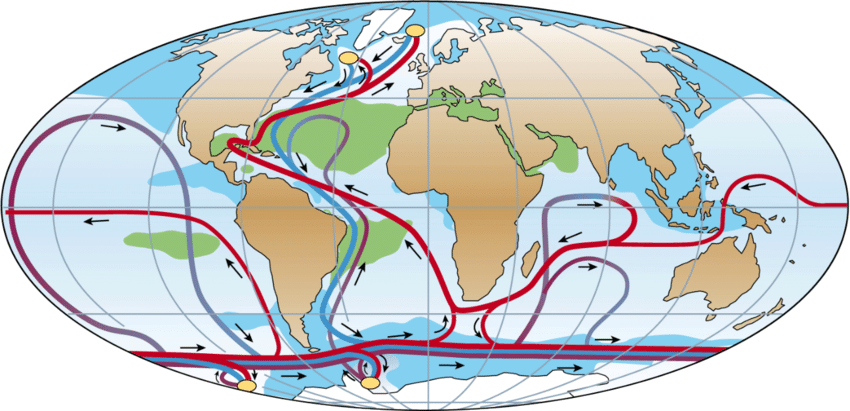
\includegraphics[width=0.4\linewidth]{Simplified-sketch-of-the-global-thermohaline-circulation-pathway-whereby-yellow-dots.png}
    %\caption{Simplified Sketch of the Global Thermohaline Circulation Pathway (Rahmstorf)}
    \label{fig:enter-label}
\end{figure}

The \emph{Stommel model} reduces the Northern Atlantic ocean to two boxes representing respectively the high-latitude (polar) region and low-latitude (tropical) region. Each of them has its own water temperature and water salinity, and there is a surface flow $q$ as pictured below:
\begin{figure}[h]
\centering
    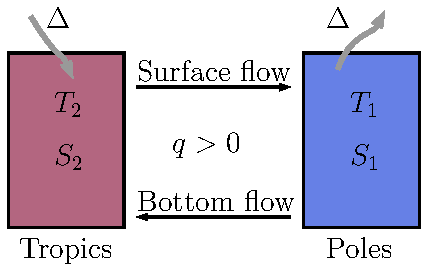
\includegraphics[width = 0.3\linewidth]{Stommel.pdf}
    \caption{The two-vessel model. The relevant parameters are the differences $T_2 - T_1$ and $S_2 - S_1$. An influx of fresh water at the poles corresponds to a decrease in salinity, represented by $\Delta$.}
    \label{fig:enter-label}
\end{figure}
When $q>0$ the flow of water on the bottom of the ocean is from high latitudes to low latitudes, which creates an equal flow on the surface of the ocean from low latitudes to high latitudes.

The flow of water $q$ depends on the differences $T_2 - T_1$ and $S_2 - S_1$ (which is itself influenced by the flux~$\Delta$) and it can be modelled by the equation
\begin{equation}
    \frac{dq}{dt} = -|q|(q - k_1) - k_2,
\end{equation}
where the positive constant $k_1$ is proportional to the difference $T_2 - T_1$ in temperature between high and low latitudes and the positive constant $k_2$ depends on $\Delta$. The key to this assignment is that \emph{an increase in glacial melting will increase $k_2$}, and we shall explore the consequences of this fact.
\begin{enumerate}
    \item Find the steady state solutions for $q$. You should consider the case where $q>0$ and the case where $q<0$ separately.  You should be able to disregard one of the solutions you find in one of the cases because of a contradiction. 
   
    \item There is a value of $k_2$ where two of the fixed points vanish completely. Find this value of $k_2$, call it $k_c$.  
  \\


    \item Determine the stability of the three steady states when $k_2<k_c$ and the stability of the one steady state when $k_2>k_c$

  


\item Plot the fixed points you found in question 1 as a function of $k_2$, so that the fixed points, $q$, are on the $y$ axis and $k_2$ is on the $x$ axis. This is called the \textit{Bifurcation Diagram} of equation (1).




\item Currently in the North Atlantic the bottom flow, $q$, is stable and positive, meaning that the bottom flow in the ocean moves from high to low latitudes and the surface flow moves from low to high latitudes. Which steady state does that mean the ocean is currently in and what does this say about the value of $k_2$?



\item Now imagine that a large amount of freshwater is moving into ocean at high-latitudes, so that $k_2>k_c$.  One example of this would be glacial melting, which would increase the freshwater input to the ocean at high latitudes.
\\
Explain what happens in the context of the system - based on the bifurcation diagram you created in the previous question. Specifically, what will happen to the sign of $q$ and what does that mean in terms of the direction of ocean flow?

 
\end{enumerate}

 \section{Analytical solution}
We can actually solve the following equation explicitly, by using two cases:
\begin{equation}
    \dfrac{dq}{dt} = -2|q|(q - k_1) - k_2, \quad q(0)=q_0.\label{eq:q}
\end{equation}
\begin{enumerate}
    \item Find an expression for $q(t)$ using separation of variables, assuming $k_2<k_c$. To solve, consider the cases when $q>0$ and $q<0$ separately. For the $q>0$ case assume $q_0>0$ and for the $q<0$ case assume $q_0<0$. Note: it will be easier to solve using partial fraction decomposition rather than using inverse trig functions. Before doing partial fractions, it may be helpful to first factor the equation in terms of the roots we already found: ($q_1, q_2$) for $q>0$, ($q_3, q_4$) for $q<0$. 
  

    \item Plot your analytical solutions you found in the previous question to confirm that their limiting behavior are correct. You can pick any $k_1>0$ and $k_2>0$ but your plots should be in the region where $k_2<k_c$. For your solution where $q<0$, plot one solution where $0<q_0<q_4$ and one solution where $q_0<q_4$ ($q_4$ is the steady state when $q<0$). For your solution where $q>0$, plot one solution when $0<q_0<q_2$, one solution where $q_2<q_0<q_1$ and one solution where $q_0>q_1$. Here $q_1$ and $q_2$ are the two positive steady states, with $q_1>q_2$.


    
    \item Plot $\dfrac{dq}{dt}$ as a function of $q$, and use this plots to draw a phase line for equation (2), still assuming $k_2<k_c$. Does the phase line agree with the limiting behaviour of your analytical solutions? 
    \item When $k_1 = k_2 = 4$, sketch all different possible trajectories. (There should be 7 trajectories, including the ones that remain on a fixed point)
\subsection{Matching Problem}
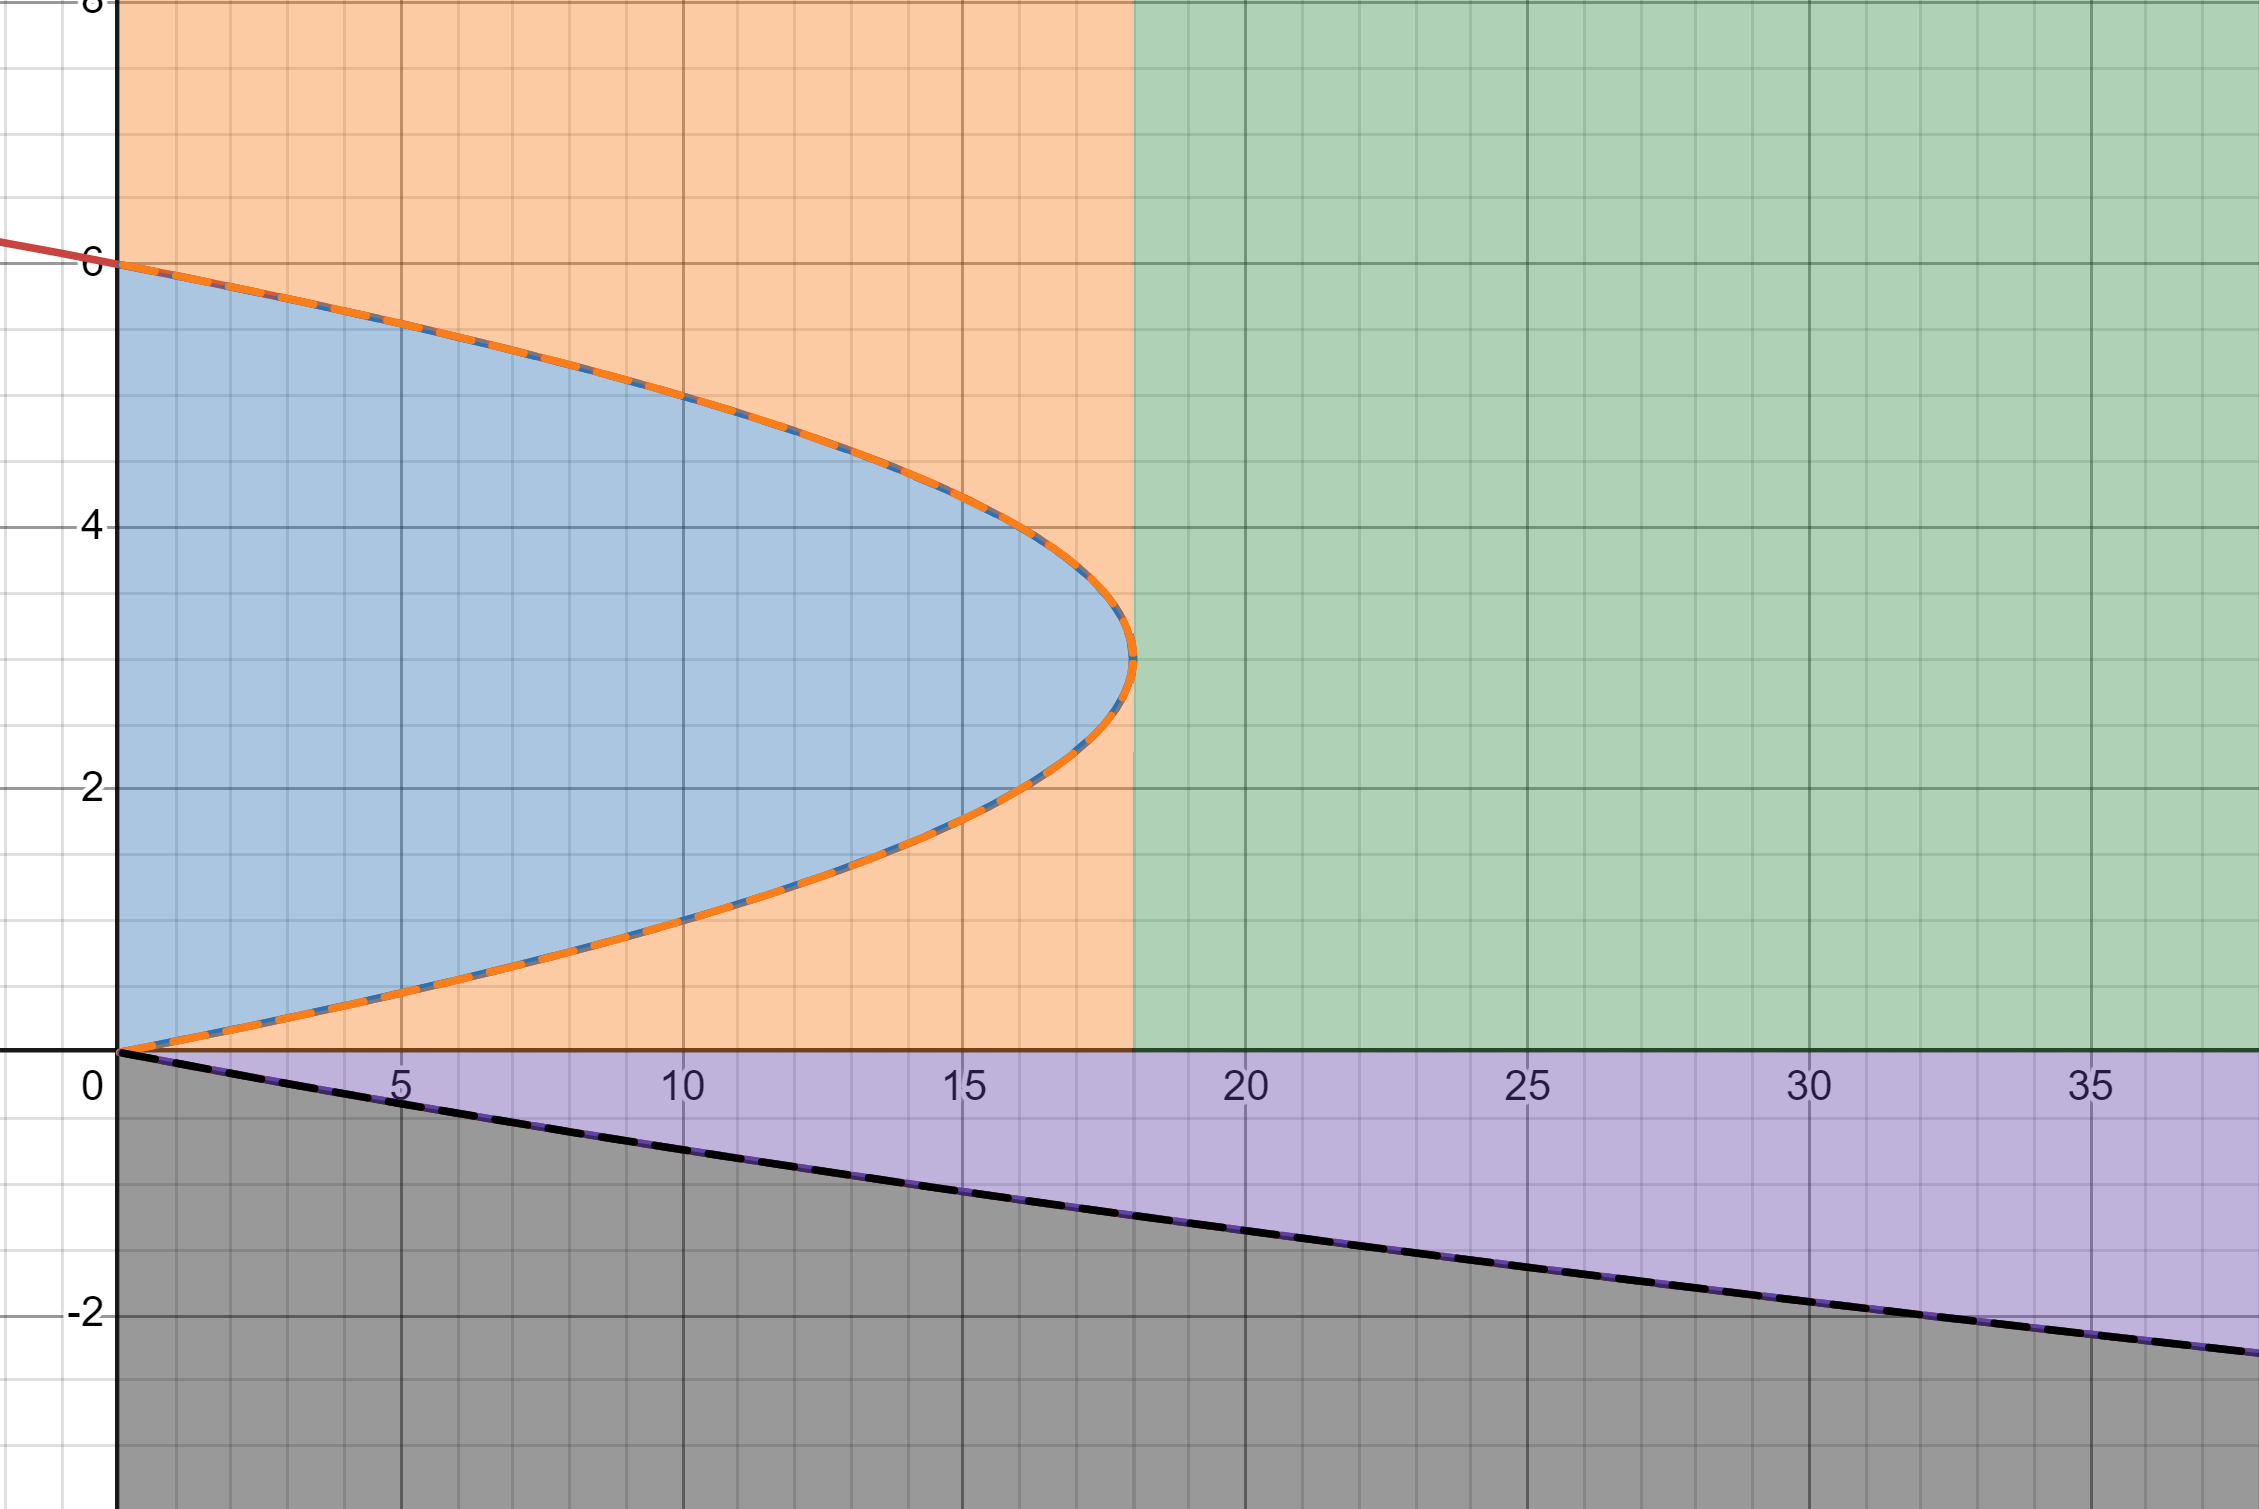
\includegraphics[width = 300pt]{2024-2025 Math 215 Assignments (in progress)/THCbifurcationdiagram.png} \\

In the previous section you found expressions for $q(t)$ when $q>0$ and $q<0$, subject to the initial condition $q_0$. However, if $0<q_0<q_2$, then the solution you found will initially be positive but will decrease over time and eventually become negative. In this section, we will demonstrate how to match the solution you found for $q>0$ with the solution you found for $q<0$ so that you have one piecewise solution that will hold for all $t$ when $0<q_0<q_2$.




Let $0<q_0<q_2$ (and $k_2<k_c$) then the solution begins in the lower orange region of the graph above. In this case, the positive solution is given by 

\begin{equation}
        q_+(t) = \dfrac{q_1(q_0 - q_2) - q_2(q_0 - q_1)e^{-2t(q_1-q_2)}}{(q_0 - q_2) - (q_0 - q_1)e^{-2t(q_1-q_2)}}.
\end{equation}

The solution in the purple region where $q<0$ is given by 

    \begin{equation}
        q_-(t) = \dfrac{q_3 - q_4ke^{2t(q_3-q_4)}}{1 - ke^{2t(q_3-q_4)}} \label{eq:q_-}
    \end{equation}
where $k$ is a constant of integration.

\item First, find the time, $t_1^*$, when $q_+(t_1^*)=0$.


\item Now use $q_+(t_1^*)=0$ as an initial condition to solve for $k$ in $q_-(t)$. You now have a continuous (piecewise) solution for $q(t)$ which holds for all $t$!



\item If instead $k_2>k_c$ and $q_0>0$, then the solution, $q(t)$ begins in the green region and is given by:

\begin{align}
    q_+(t) &= \sqrt{\frac{k_2}{2} - (\frac{k_1}{2})^2}\tan(\sqrt{2k_2 - k_1^2}(-t + c)) + \frac{k_1}{2},\\
    c&=\frac{\arctan\left(\frac{q_0-\frac{k_2}{2}}{\sqrt{\frac{k_2}{2}-\frac{k_1^2}{4}}}\right)}{2k_2-k_1^2}
\end{align}
when $q>0$. The solution will then move into the purple region, where the analytical expression is given in equation \ref{eq:q_-}. Find a \textbf{different} $k$ in $q_-(t)$ so that the solution, $q(t)$ is continuous for all $t$ in this parameter regime. Note: as before, you will first need to find the time $t_2^*$ when $q_+(t_2^*)=0.$




\subsection{Asymptotics}
Now that we have found the explicit form of the solutions, we'll look into the limiting behavior. 
\item Find $\displaystyle \lim_{t\to \infty} q(t)$, when $q_0<0$.

\item 
Recall that 
\begin{equation}
    q_+(t) = \dfrac{q_1(q_0 - q_2) - q_2(q_0 - q_1)e^{-2t(q_1-q_2)}}{(q_0 - q_2) - (q_0 - q_1)e^{-2t(q_1-q_2)}}.
\end{equation}
This is the solution to (\ref{eq:q}) when $q_0>0$ and $k_2<k_c$. Remember that $q_1$ and $q_2$ are the two positive steady states, with $q_1>q_2$.

Find $\displaystyle \lim_{t\to\infty}q_+(t)$ when 
\begin{enumerate}
\item $q_1<q_0$

\item $q_2<q_0<q_1$

\item $q_0<q_2$

\item $0<q_0<q_2$

\end{enumerate}


    
\subsection{Conceptual Questions}
We can plot this ODE computationally - and for specific parameter values we observe interesting behaviour. Consider two different graphs for different $k_2$: $k_1 = 2, k_2 = 2$ and $k_1 = 2, k_2 = 2.5$. \\
\begin{figure} [h]
    \centering    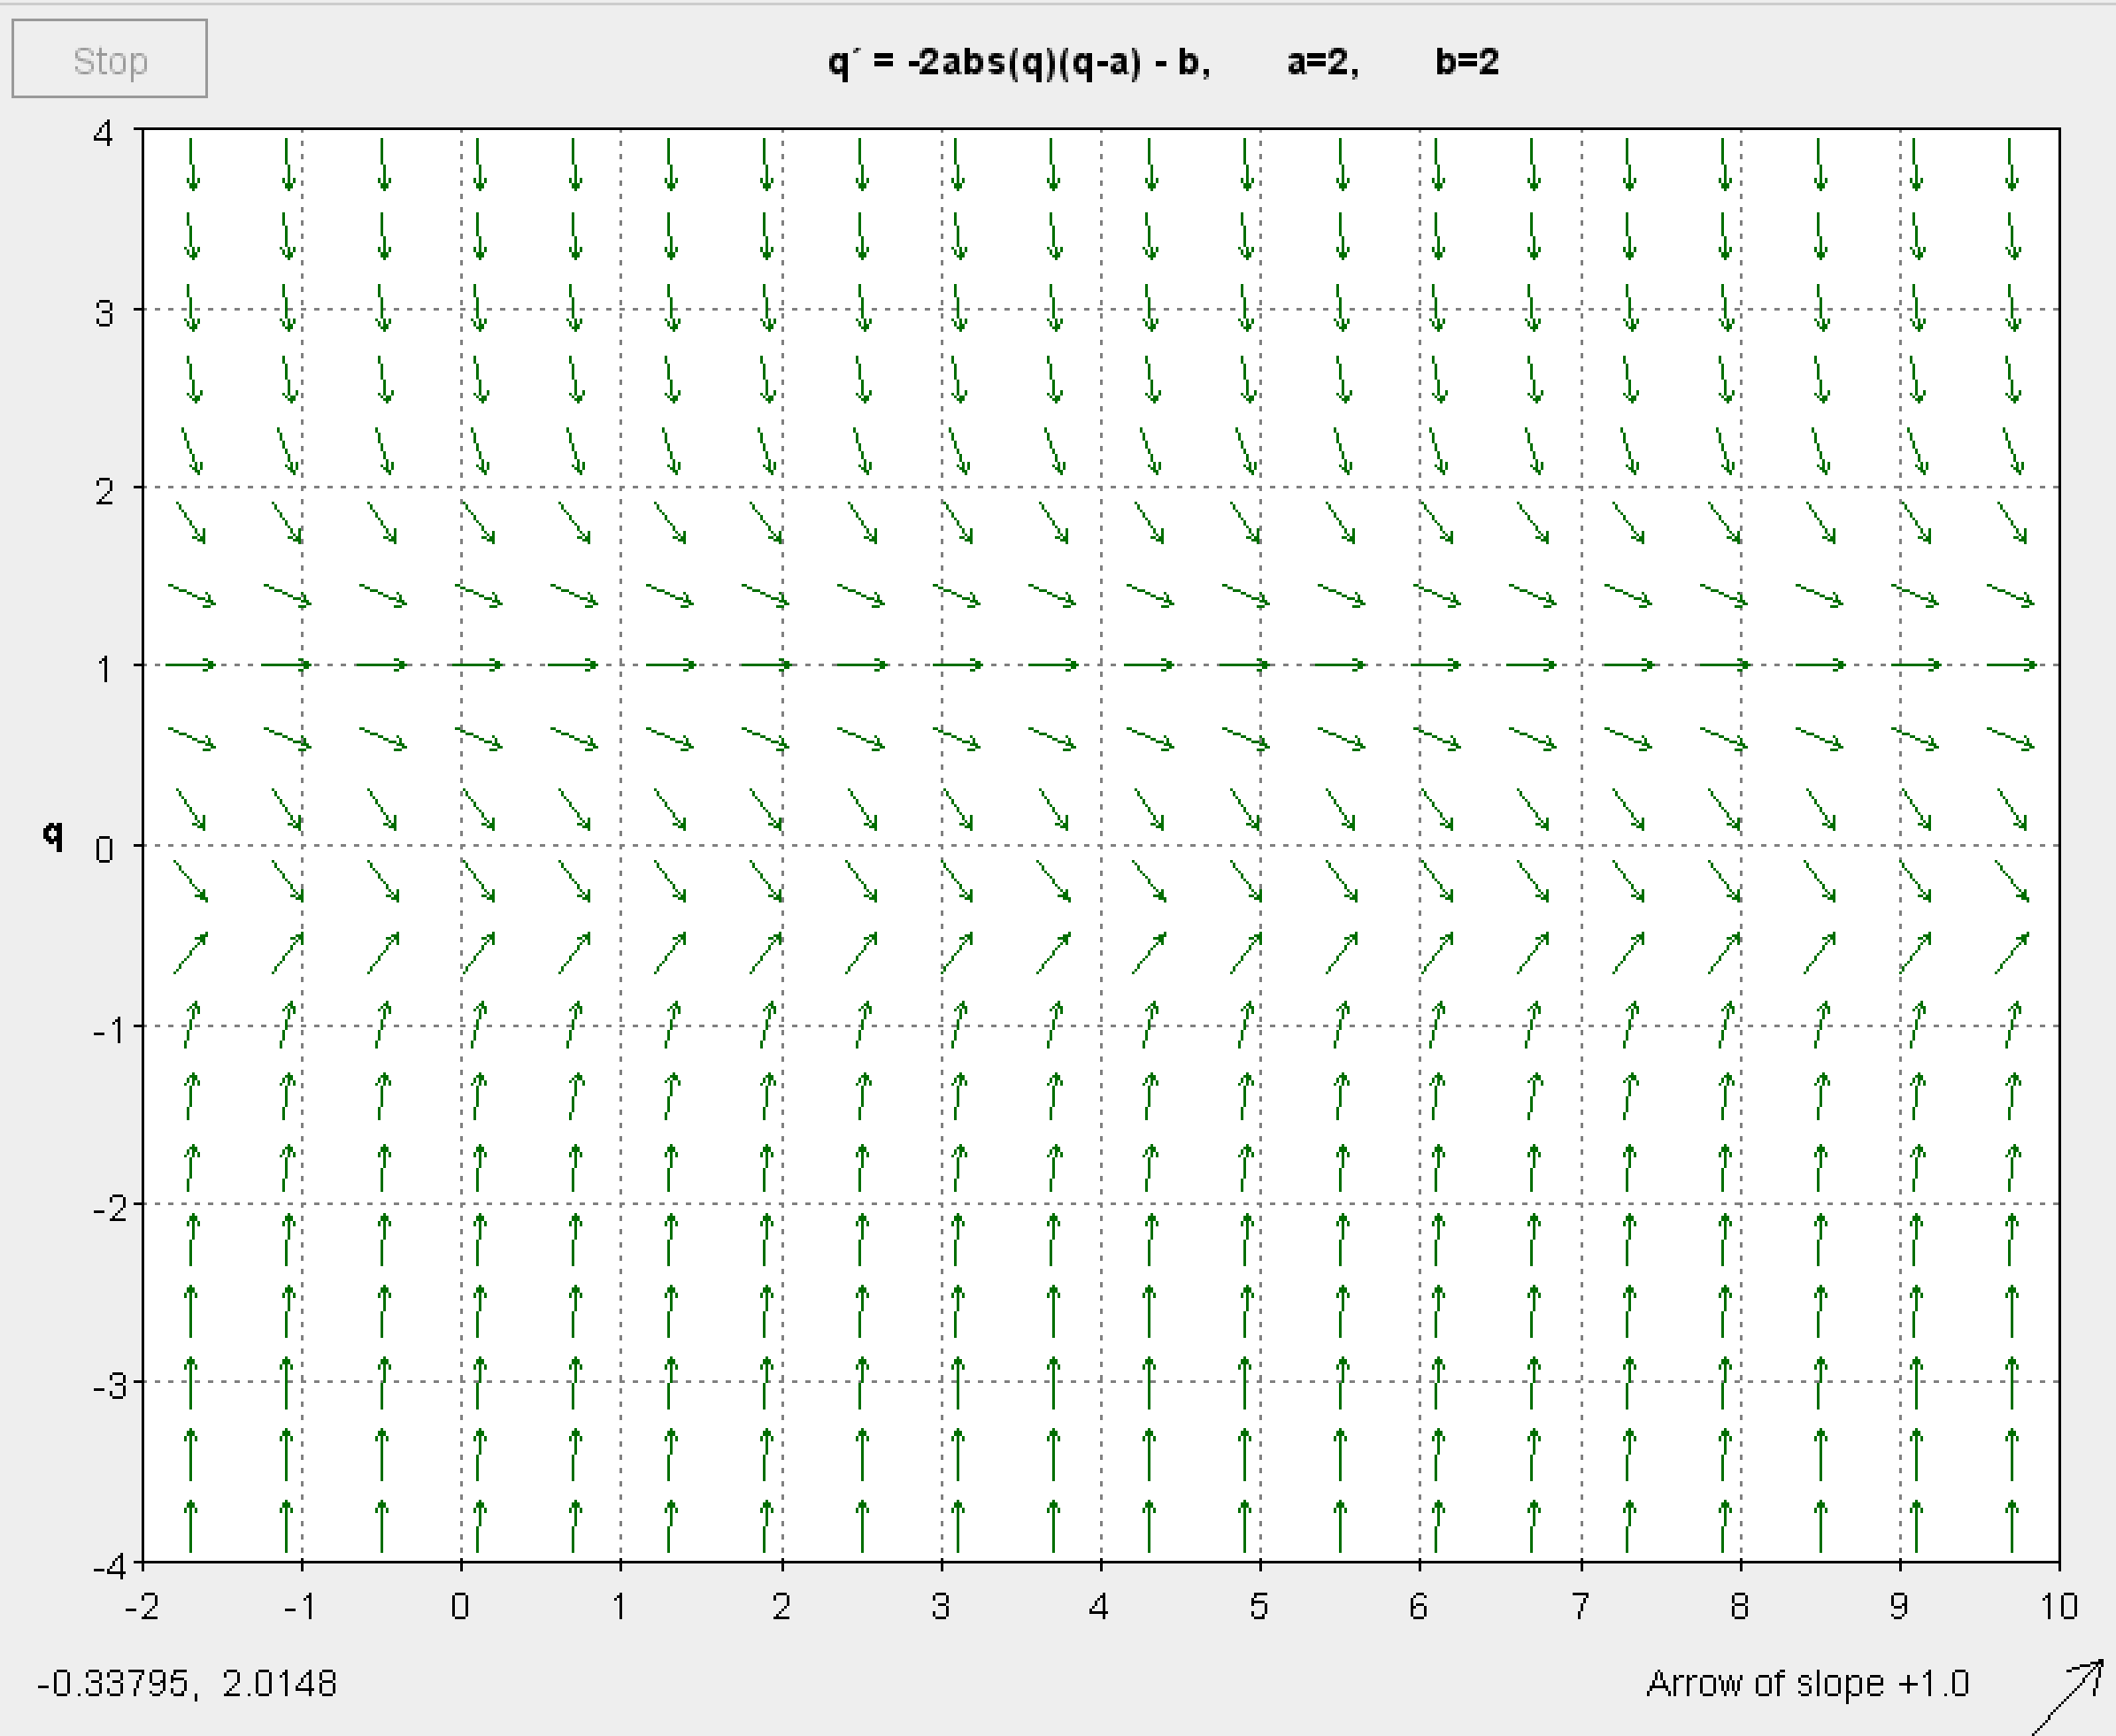
\includegraphics[width=0.5\linewidth]{2024-2025 Math 215 Assignments (in progress)/a=2,b=2.png}
    \caption{$k_1 = 2, k_2 = 2$}
    \label{fig:enter-label}
\end{figure} \\
\begin{figure} [h]
    \centering    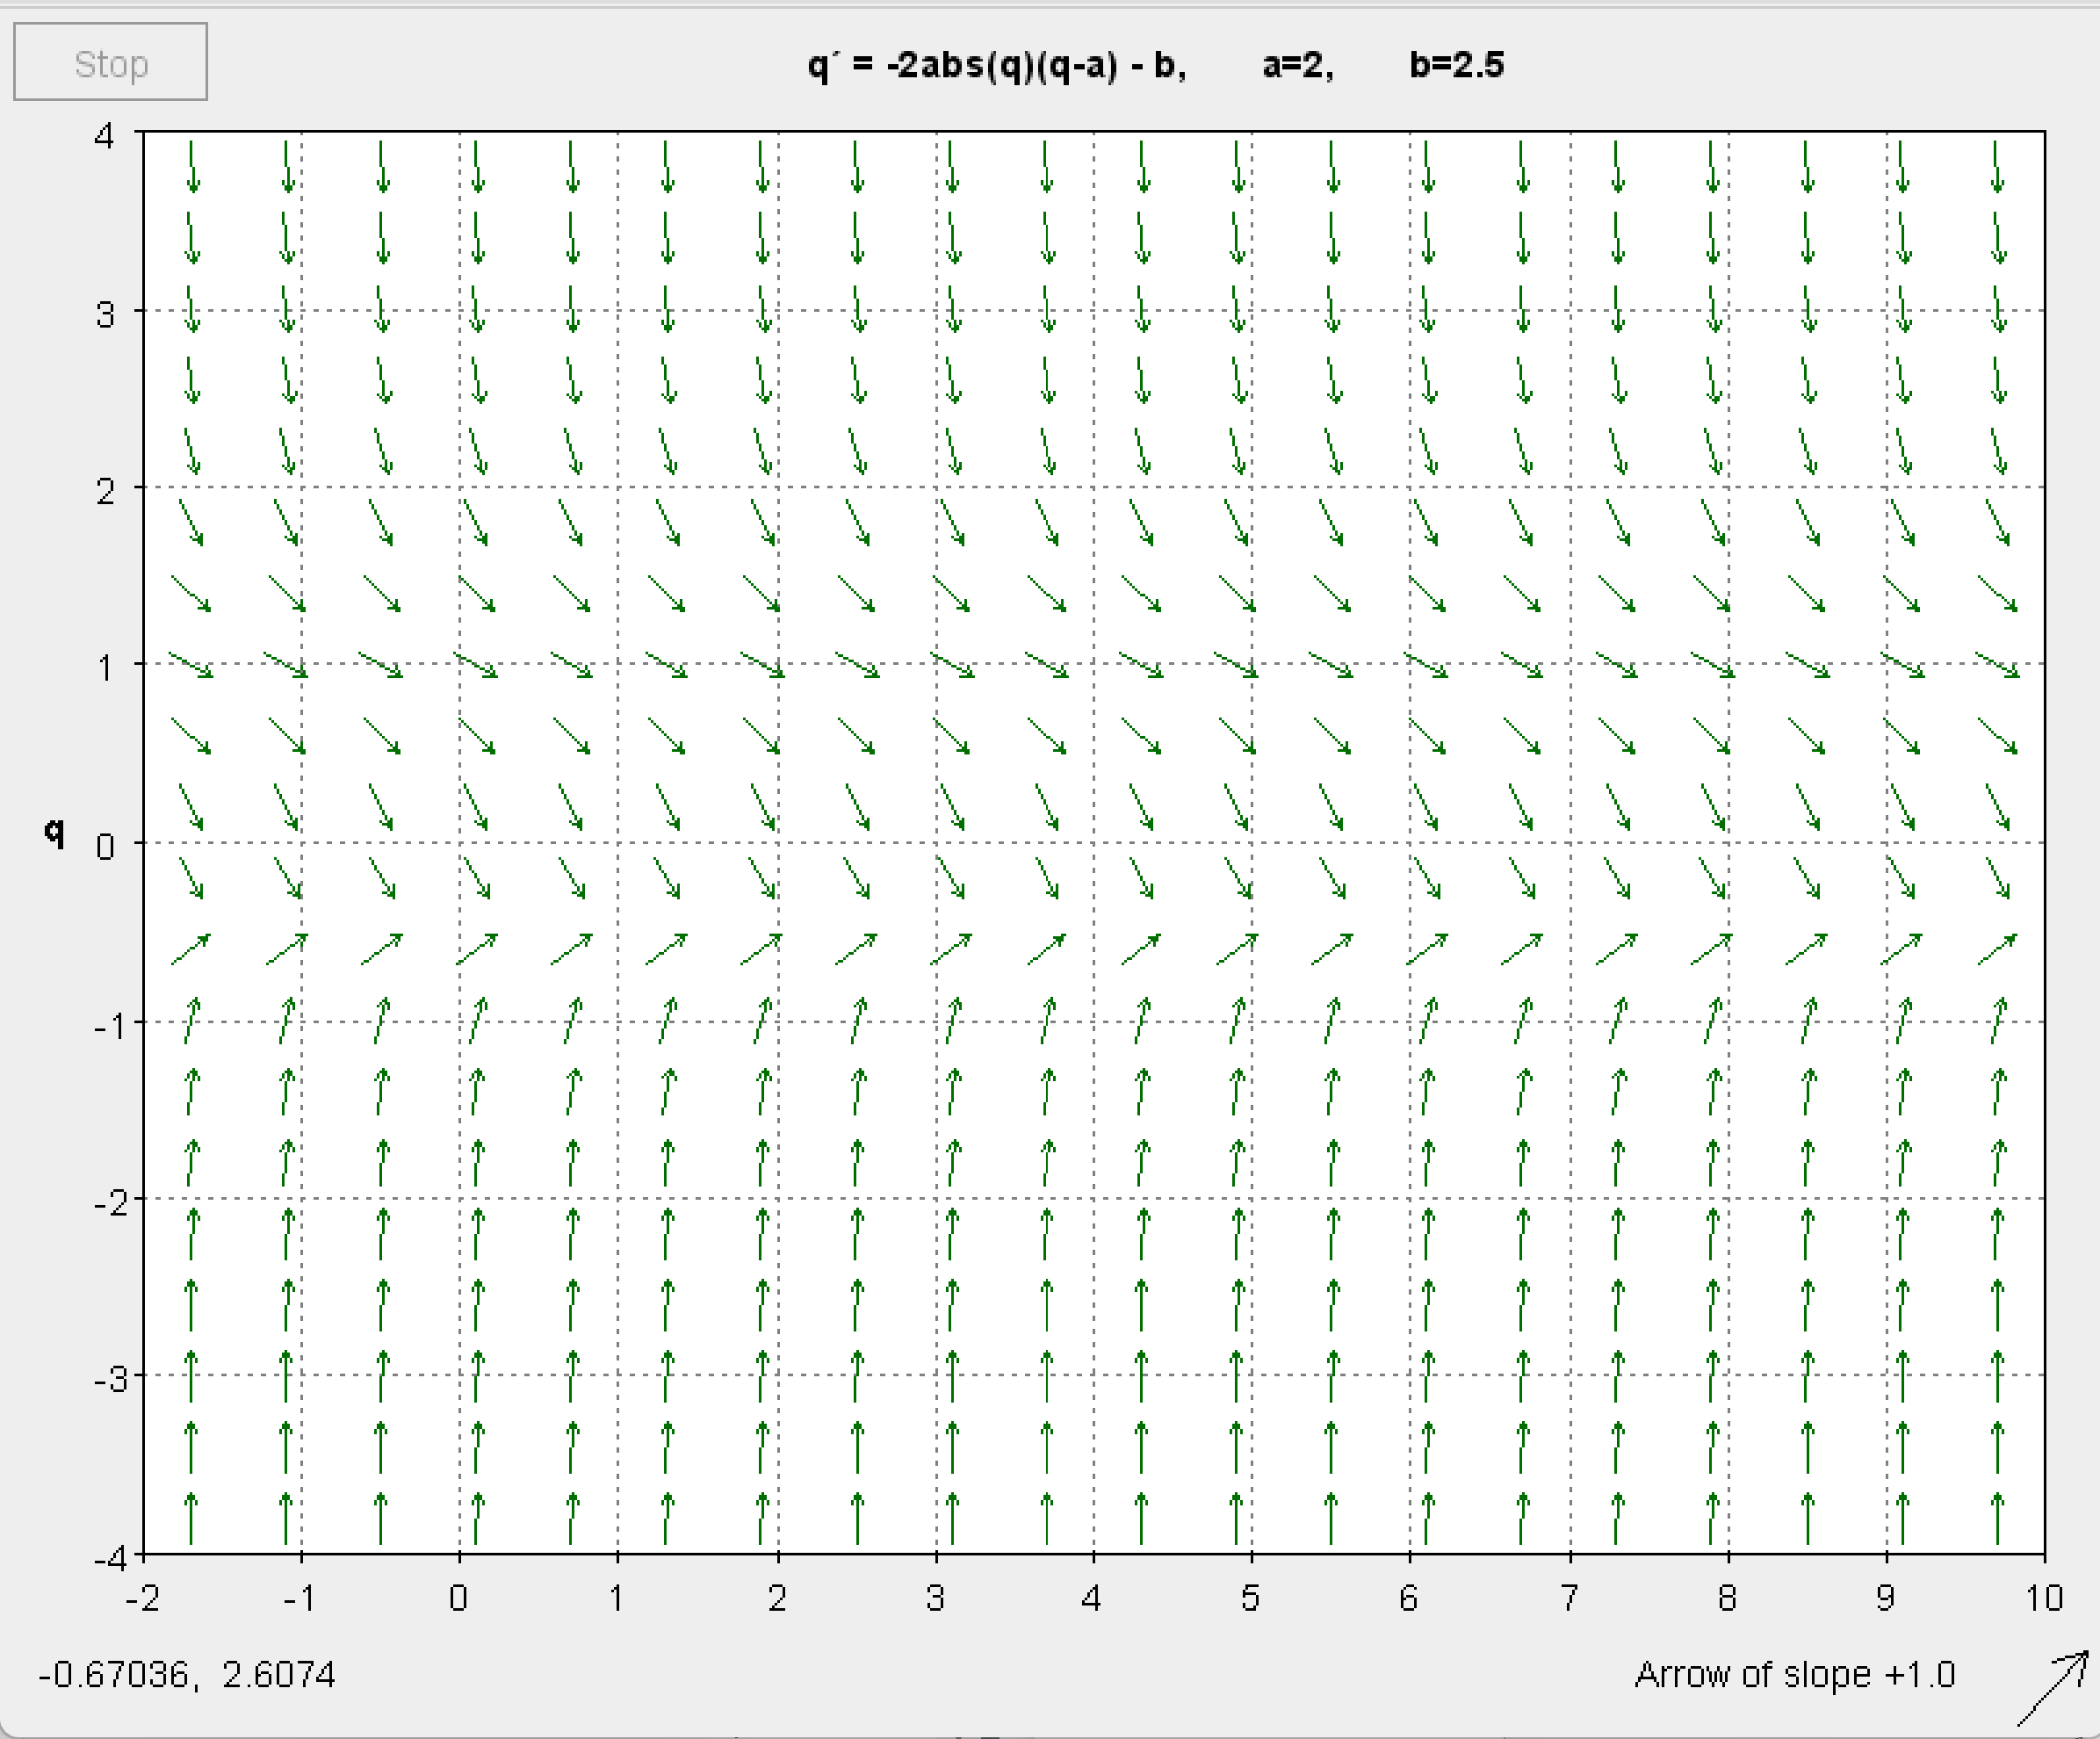
\includegraphics[width=0.5\linewidth]{2024-2025 Math 215 Assignments (in progress)/a=2,b=2.5.png}
    \caption{$k_1 = 2, k_2 = 2.5$}
    \label{fig:enter-label}
\end{figure} \newpage
\item Sketch out all qualitatively different trajectories on both graphs (when $k_2 = 2$, and $k_2 = 2.5$). 
\item Explain why the second graph has a section where the trajectories shift to the right slightly around $q=1$, rather than continuing downwards uniformly.

\item Explain what this change in solution behavior means in the context of the physical climate system.

\end{enumerate}

\begin{thebibliography}{9}
\bibitem{figure}
Kaper, H. G, and Hans Engler. \emph{Mathematics and Climate}. Philadelphia, Pennsylvania: Society for Industrial and Applied Mathematics SIAM, 3600 Market Street, Floor 6, Philadelphia, PA 19104, 2013. Print.

\bibitem{boxmodel}
Marotzke, Jochem. \emph{Abrupt Climate Change and Thermohaline Circulation}. PNAS, 15 Feb. 2000. \\
\url{www.pnas.org/doi/full/10.1073/pnas.97.4.1347} 

\bibitem{thcpathway}
Rahmstorf, Stefan. \emph{The Thermohaline Ocean Circulation}. Potsdam Institute for Climate Research. \\
\url{www.pik-potsdam.de/~stefan/thc_fact_sheet.html}

\end{thebibliography}
\end{document}